
\usetikzlibrary{positioning}
\definecolor{red}{HTML}{8A3F3A}
\definecolor{yellow}{HTML}{E0BB3C}
\definecolor{blue}{HTML}{4569E0}
\definecolor{green}{HTML}{17E561}
\definecolor{other}{HTML}{6A939E}

% DTU Colors
\definecolor{dtu-corporate-red}{HTML}{990000}
\definecolor{dtu-white}{HTML}{ffffff}
\definecolor{dtu-black}{HTML}{000000}
\definecolor{dtu-blue}{HTML}{2F3EEA}
\definecolor{dtu-bright-green}{HTML}{1FD082}
\definecolor{dtu-navy-blue}{HTML}{030F4F}
\definecolor{dtu-yellow}{HTML}{F6D04D}
\definecolor{dtu-orange}{HTML}{FC7634}
\definecolor{dtu-pink}{HTML}{F7BBB1}
\definecolor{dtu-grey}{HTML}{DADADA}
\definecolor{dtu-red}{HTML}{E83F48}
\definecolor{dtu-green}{HTML}{008835}
\definecolor{dtu-purple}{HTML}{79238E}


\newlength{\basisordinatorcratestructure}
\setlength{\basisordinatorcratestructure}{0.3cm}
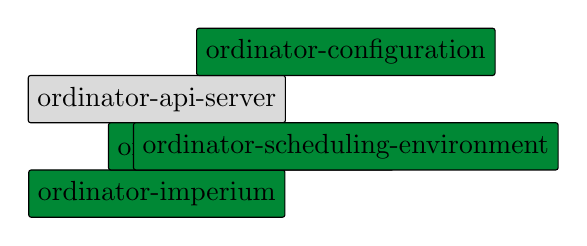
\begin{tikzpicture}[xshift=-3cm]
    \draw (-4.0\basisordinatorcratestructure,4.0\basisordinatorcratestructure) 
		node[minimum height=2\basisordinatorcratestructure,fill=dtu-grey,minimum width=3\basisordinatorcratestructure,draw, rounded corners=0.1\basisordinatorcratestructure] 
			(ordinator-api-server) {ordinator-api-server};

    \draw (-4.0\basisordinatorcratestructure,0.0\basisordinatorcratestructure) 
		node[minimum height=2\basisordinatorcratestructure,fill=dtu-green,minimum width=3\basisordinatorcratestructure,draw, rounded corners=0.1\basisordinatorcratestructure] 
			(ordinator-imperium) {ordinator-imperium};

    \draw (0.0\basisordinatorcratestructure,2.0\basisordinatorcratestructure) 
		node[minimum height=2\basisordinatorcratestructure,fill=dtu-green,minimum width=3\basisordinatorcratestructure,draw, rounded corners=0.1\basisordinatorcratestructure] 
			(ordinator-orchestrator) {ordinator-orchestrator};

    \draw (4.0\basisordinatorcratestructure,2.0\basisordinatorcratestructure) 
		node[minimum height=2\basisordinatorcratestructure,fill=dtu-green,minimum width=3\basisordinatorcratestructure,draw, rounded corners=0.1\basisordinatorcratestructure] 
			(ordinator-scheduling-environment) {ordinator-scheduling-environment};

    \draw (4.0\basisordinatorcratestructure,6.0\basisordinatorcratestructure) 
		node[minimum height=2\basisordinatorcratestructure,fill=dtu-green,minimum width=3\basisordinatorcratestructure,draw, rounded corners=0.1\basisordinatorcratestructure] 
			(ordinator-configuration) {ordinator-configuration};


	% \draw[<->, thick, line width=0.1\basisordinatorcratestructure] (Planner) -- (Scheduler);
	% \draw[<->, thick, line width=0.1\basisordinatorcratestructure] (Scheduler) -- (Supervisor_3);
	% \draw[<->, thick, line width=0.1\basisordinatorcratestructure] (Supervisor_3) -- (Technician_5);
	% \draw[<->, thick, line width=0.1\basisordinatorcratestructure] (Scheduler) -- (Database);
	% \draw[<->, thick, line width=0.1\basisordinatorcratestructure] (Scheduler) -- (UserInterface);
\end{tikzpicture}
